\documentclass[12pt, preprint]{aastex}
%\documentclass{emulateapj}
\usepackage{apjfonts,graphicx,here,common,longtable,ifthen,amsmath,amssymb,natbib,lscape}
\usepackage[pagebackref,
  pdftitle={},
  pdfauthor={},
  pdfsubject={Astrophysics},
  pdfkeywords={},
  pdfproducer={LaTeX with hyperref},
  pdfcreator={LaTeX}
  pdfdisplaydoctitle=true,
  colorlinks=true,
  citecolor=blue,
  linkcolor=blue,
  urlcolor=blue]{hyperref}
\bibliographystyle{apj}
\begin{document}

\section{Dust}

Using \textsc{ellipse} routine in IRAF the surface brightness profile
of MS0735 was derived. Using the information deduced by this routine a
model galaxy was created using \textsc{bmodel}. This model is assumed
to be a pure light model (\ie\ no extinction). Using the radiative
transfer equation,
\begin{equation}
  e^{-\tau} = \frac{I(r)}{I_0(r)}
\end{equation}
the observed image and the model image, an optical depth image was
created. Here the observed image is $I(r)$, the model image is
$I_0(r)$ and the tau image was created by performing the
following arithmetics on the images.
\begin{equation}
  \tau = ln~\frac{I_0(r)}{I(r)}
\end{equation}

\begin{figure}[ht]
  \begin{center}
    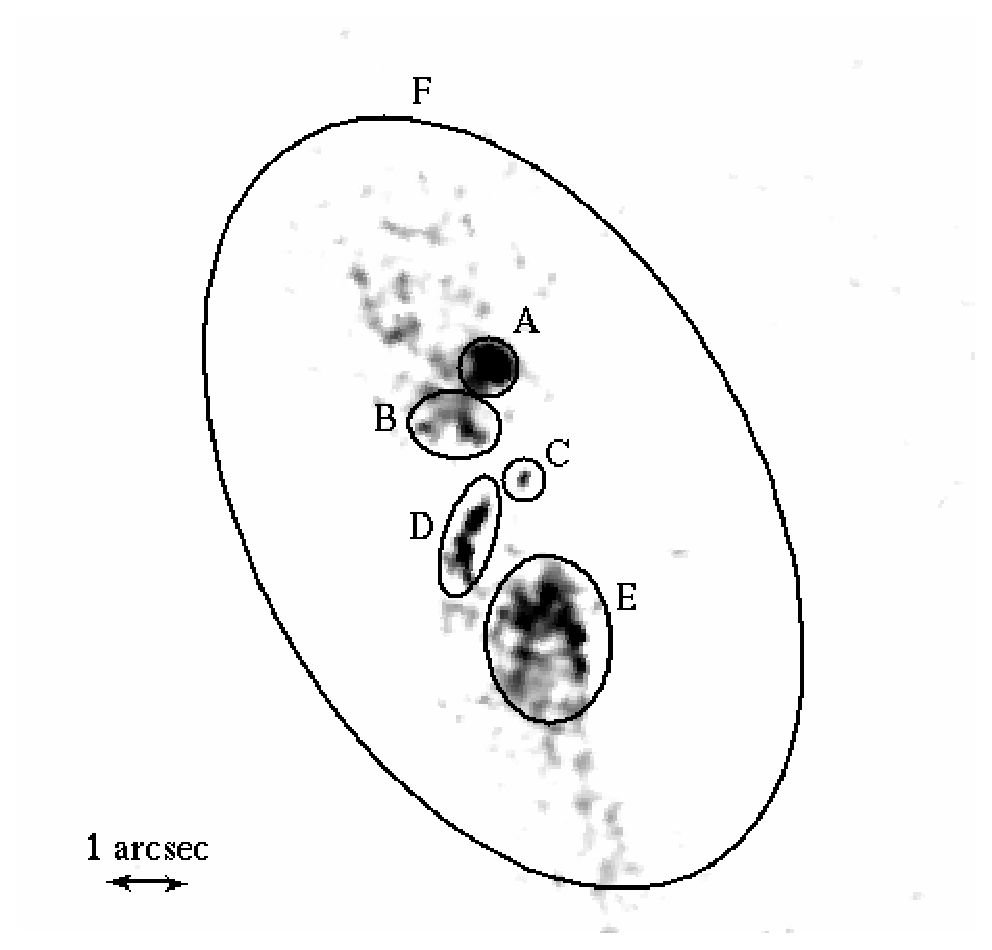
\includegraphics[width=0.5\textwidth]{dustregion.eps}
    \caption{Residual map of Herc A after subtraction of the model
      galaxy. Regions of high extinction have been chosen for dust
      calculation.}
  \end{center}
\end{figure}

\begin{deluxetable}{lcccc}
  \tabletypesize{}
  \tablecaption{Measurement of gas and dust mass in Herc A using the optical depth.}
  \tablewidth{0pt}
  \tablehead{
    \colhead{} & Area of Region & {} & $N_{H}$  & Total Gas Mass \\
    Region & $(10^{43}$ $cm^{2})$ & $<\tau>$\tablenotemark{a} & $(10^{20})$ & $(10^{6}$ $M_{\sun}$)  \\ }
  \startdata
  A 	& 2.27	& 0.341$\pm$0.128		& 7.02$\pm$2.64	& 13.5$\pm$5.06\\
  B	& 3.31	& 0.149$\pm$0.047		& 3.06$\pm$0.961	& 8.57$\pm$2.69\\
  C	& 0.23	& 0.178$\pm$0.034		& 3.66$\pm$0.698	& 0.712$\pm$0.25\\
  D	& 0.14	& 0.212$\pm$0.069		& 4.37$\pm$1.43	& 5.17$\pm$1.69\\
  E 	& 10.16	& 0.187$\pm$0.062		& 3.86$\pm$1.27	& 33.1$\pm$10.9\\
  F	& 71.19	& 0.331$\pm$0.075		& 6.81$\pm$1.55	& 276.5$\pm$62.65\\
  \enddata
  \tablecomments{The uncertainty in measured quantities are derived using Poisson statistics combined with the statistical error.}
  \tablenotetext{a}{Optical Depth.}
\end{deluxetable}

\section{SFR}

We used XMM-Newton Optical Monitor, Ultraviolet (UV) images to
determine a star formation rate (SFR) for Herc A. The data were
retrieved from the online XMM archives in MAST (Multimission Archive
at STScI) . We retrieved XMM-OM Medium 2 (M2) with 13.77 ks exposure
time and Wide 1 (W1) with 5 ks exposure time. The properties of these
filters are listed in the table below. Recently \citet{salim2007}
proposed a relationship which estimates the SFR using UV luminosities.
\begin{equation}
  SFR(\msolpy) = 1.4 \times 10^{-28} ~L_{\nu} ~\ergpshz
\end{equation}
The luminosity of the UV images were determined in apertures at radii
of multiples of the PSF for each filter. The total count rate (cps)
within an aperture was measured and a frequency normalized luminosity
was calculated. This in turn allowed for the SFR calculations using
equation (1).
\begin{equation}
  F = F_{\circ} \lambda c_r ~\flux
\end{equation}
where $c_r$ is the count rate per second,
\begin{equation}
  L = F 4\pi \dl^2 ~\lum
\end{equation}
\begin{equation}
  L_{\nu} = \frac{L \lambda}{c} ~\ergpshz
\end{equation}
It is noted that the SFRs measured for all images are upper limits,
i.e. no detections were made, except for 5 ks exposure using the
XMM-OM Wide 1 filter. In this image a minimal detection is made. In
this image a minimal detection is made which is several times the PSF
of the filter (fig. below). An ultraviolet luminosity and a star
formation rate of $1.16 ~(\pm 0.16) \times 10^{42} ~\lum$, $0.157 \pm
0.022 ~\msolpy$ respectively in an aperture of 10\arcs.

\begin{figure}[h]
  \begin{center}
    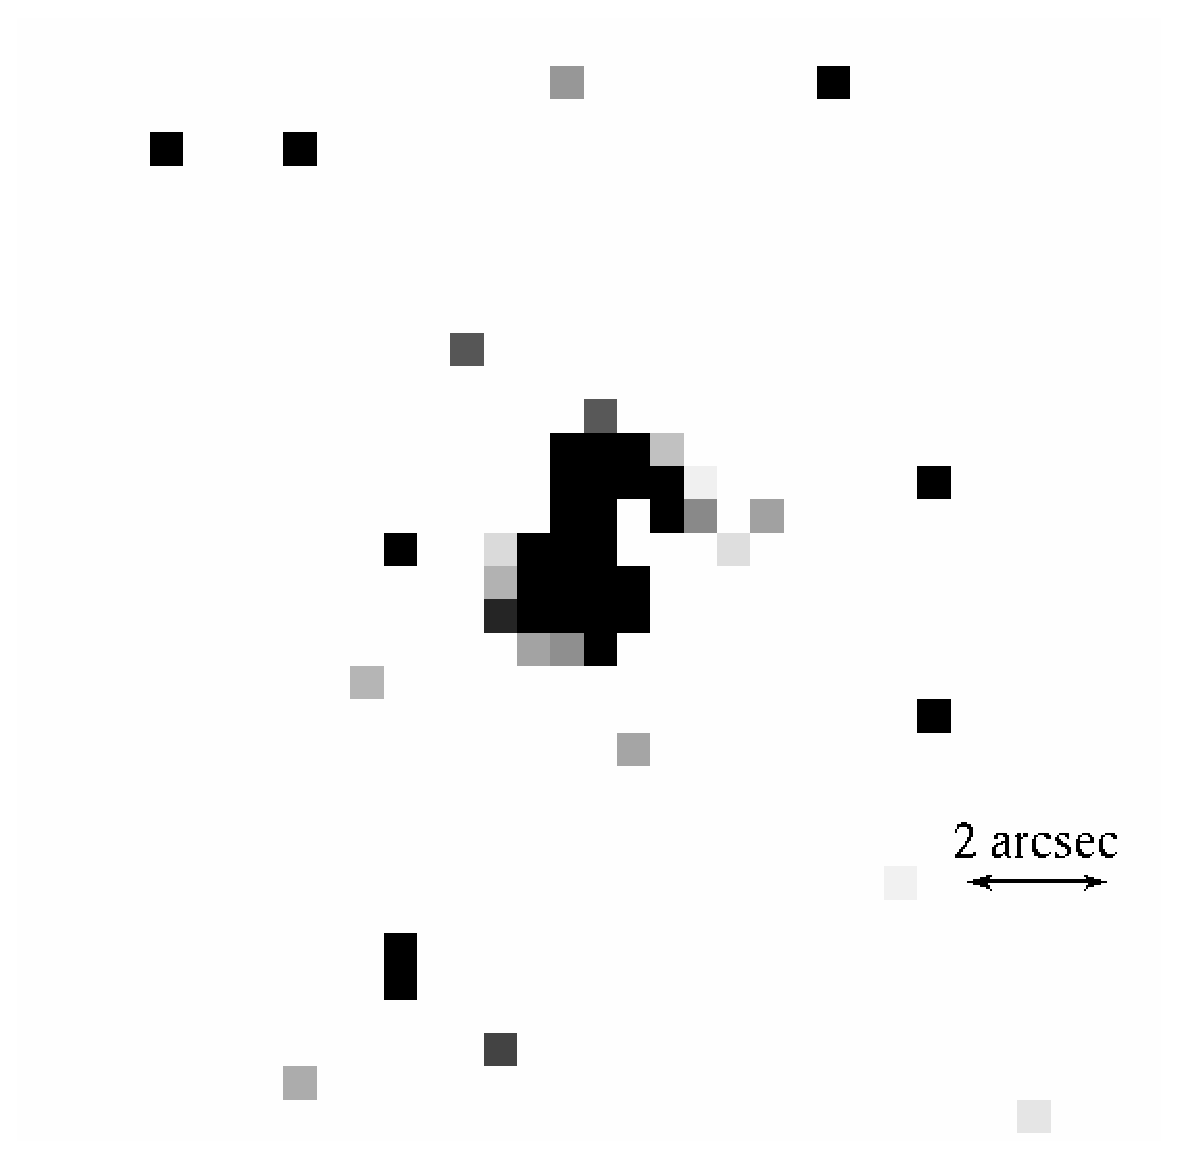
\includegraphics[width=0.5\textwidth]{xmmw1.eps}
    \caption{XMM-OM Wide 1 long exposure image shows a faint UV detection
      of Herc A. The color map is inverted in this image.}
  \end{center}
\end{figure}

\begin{deluxetable}{lcccc}
  \tabletypesize{}
  \tablecaption{Properties of the Ultraviolet observations.}
  \tablewidth{0pt}
  \tablehead{
    \colhead{} & Central Wavelength & $m_{\circ,AB}$ & PSF & $F_{\circ}$ \\
    Filter & $(\AA)$ & {} & (arcsecs) & (ergs/s/$cm^{2}/\AA$/cps)  \\ }
  \startdata
  M2	& 2310	& 17.41	& 1.8		& 2.20 $\times$ $10^{-15}$	\\
  W1	& 2910	& 18.57	& 2		& 4.76 $\times$ $10^{-16}$	\\
  \enddata
\end{deluxetable}

\section{HST Observation}

Our data was obtained from the HST archives on MAST. It is a 864
second exposure of Herc A using the STIS broadband 50CCD filter with
central wavelength of 5850$\AA$ with standard zero point magnitude of
26.518. The plate scale of 0.051" per pixel corresponds to an angular
size of 2.67 kpc per arcsecond at the redshift of Herc A. The
following corrections were applied to the zero point magnitude: extcor
(0.0924), kcor (0.309), evolucor (-0.191), fluxcor (0.622).

\begin{figure}[h]
  \begin{center}
    \epsscale{1}
    \plottwo{acore.eps}{score.eps}
    \caption{Inverted color map of Herc A. Left panel: Herc A with its
      companion galaxy, the dust lanes are visible in lighter color. Right
      panel: The dust lanes of Herc A, with the radio outburst direction
      noted.}
  \end{center}
\end{figure}

\bibliography{cavagnolo}

\end{document}

